\documentclass{beamer}
\usepackage{../common_slides}
\usepackage{tikz}
\usepackage{tikz-qtree}
\usepackage{pdfpages}


\usetikzlibrary{bayesnet,matrix}
% \usepackage{enumitem}
\tikzstyle{hid}=[draw]
\tikzstyle{obs}=[draw]


\title{Neural Question Answering}
\date{}
\author{CS 287}

\begin{document}
\begin{frame}
  \titlepage
\end{frame}

\begin{frame}{Review: Pooling}
  One common class of operations in neural network models is known as
  \textit{pooling}. Informally a pooling layer consists of aggregation
  unit, typically unparameterized, that reduces the input to a smaller
  size.
  \air

  Consider three pooling functions of the form $f: \reals^n \mapsto \reals$,
  \begin{enumerate}
  \item $ f(\boldx) = \max_{i} x_i $
  \item $ f(\boldx) = \min_{i} x_i $
  \item $ f(\boldx) = \sum_i x_i / n $
  \end{enumerate}
  \air

  % What action do each of these functions have? What are their gradients?
  % How would you implement backpropagation for these units?
\end{frame}

\begin{frame}{Review: Neural MT}
  Variable-length source encoding vectors from (bi)-LSTM,
  \[ \bolds_1^s, \bolds_2^s, \ldots \bolds_n^s \] 
  
  Want to construct single vector $\bolds^s_{pool}$.
  \air 


  However we also have $\bolds^t$, last RNN state 
  \air 

  \begin{enumerate}
  \item Could use standard naive average pooling.
    \air
  \item Could use current context to help out.
  \end{enumerate}
\end{frame}


\begin{frame}{Average Pooling}
  Variable-length source encoding vectors from (bi)-LSTM,
  \[ \bolds_1^s, \bolds_2^s, \ldots \bolds_n^s \] 

  \begin{itemize}
  \item Average pooling (expectation under uniform: $\alpha_j = \frac{1}{n}$)
    \[ f(\bolds^s) = \sum_{j=1}^n \frac{1}{n} \bolds_j^s = \sum_{j=1}^n \alpha_j \bolds_j^s \] 
  \end{itemize}

  \begin{center}
    \includegraphics[width=5cm]{poolavg}
  \end{center}
\end{frame}


\begin{frame}{Hard-Attention Pooling}
  % Variable-length source encoding vectors from (bi)-LSTM,
  % \[ \bolds_1^s, \bolds_2^s, \ldots \bolds_n^s \] 

  Compute score to determine selection of pooling,

  \[ z_j = s(\bolds^s_j, \bolds^t) = \tanh ([ \bolds^t,  \bolds^s_j ] \boldW + \boldb)   \] 
  \[ j^* = \argmax_{j} z_j \]

  \begin{itemize}
  \item Selection pooling (expectation under one-hot:  $\alpha_j = \delta(j = j^*)$)
    \[ f(\bolds^s) =  \bolds_{j^*}^s = \sum_{j=1}^n \alpha_j \bolds_j^s \] 
  \end{itemize}
  \begin{center}
    \includegraphics[width=5cm]{poolone}
  \end{center}

\end{frame}


\begin{frame}{Attention-Based Pooling}
  % Variable-length source encoding vectors from (bi)-LSTM,
  % \[ \bolds_1^s, \bolds_2^s, \ldots \bolds_n^s \] 

  Compute score to determine selection of pooling,

  \[ z_j = s(\bolds^s_j, \bolds^t) = \tanh ([ \bolds^t,  \bolds^s_j ] \boldW + \boldb)   \] 

  \begin{itemize}
  \item Selection pooling (expectation under softmax: $\balpha = \softmax(\boldz)$)
    \[ f(\bolds^s) =  \sum_{j=1}^n \alpha_j \bolds_j^s \] 
  \end{itemize}
  \begin{center}
    \includegraphics[width=5cm]{poolatten}
  \end{center}

\end{frame}

\begin{frame}{Recall: Dynamic Skip-Connections}
  \begin{eqnarray*}
    NN_{sl2}(\boldx) &=& (1-t) \relu(\boldx \boldW^1 + \boldb^1) + t \boldx \\
    t &=& \sigma(\boldx \boldW^t + b^t) \\
    \boldW^1 &\in& \reals^{\dhid \times \dhid} \\
    \boldW^t &\in& \reals^{\dhid \times 1} 
  \end{eqnarray*}


    %   \begin{center}
    %   \scalebox{0.7}{
    %     \begin{tikzpicture}
    %       \Tree [ .\node{$\boldh_n$}; [ .\node{$\boldh_{n-1}$}; [
    %       .$\ldots$ [ .\node(hc){$\boldh_3$}; [ .\node(hb){$\boldh_2$}; [
    %       .\node(ha){$\boldh_1$}; \node(x){$\boldx$}; ] ] ] ] ] ]
    %       \draw[dashed] (x) edge[bend left] (hb);
    %       \draw[dashed] (ha) edge[bend right] (hc);
    %     \end{tikzpicture}
    %   }
    % \end{center}

    \begin{itemize}
    \item Here attention is between keeping state and updating.
    \end{itemize}
  \begin{center}
    \includegraphics[width=5cm]{pooldyn}
  \end{center}
\end{frame}

% \begin{frame}{Recall: Dynamic Skip-Connections}
%   \begin{eqnarray*}
%     NN_{sl2}(\boldx) &=& (1-t) \relu(\boldx \boldW^1 + \boldb^1) + t \boldx \\
%     t &=& \sigma(\boldx \boldW^t + b^t) 
%   \end{eqnarray*}


%   \begin{eqnarray*}
%      \frac{\partial L}{\partial h_{n-1,j_{n-1}} }  =  &(1-t)& (\sum_{j_n}   \indicator(h_{n, j_n} > 0) W_{j_{n-1},j_n} \frac{\partial L}{\partial h_{n, j_n}}) \\
%     + &t& ( h_{n-1, j_{n-1}} \frac{\partial L}{\partial h_{n, j_{n-1}}}) + \ldots \\ 
%   \end{eqnarray*}

%   \begin{itemize}
%   \item Note: $\boldh$ and $\boldW^t$ are also receiving gradients through the sigmoid!
%     \air
%   \item (Backprop is fun.)
%   \end{itemize}
% \end{frame}


\begin{frame}{Soft  versus Hard Pooling}
  ``Soft'' attention-based Pooling 
  \begin{itemize}
  \item Can backprop through to learn params.
  \item Allows combination of elements. 
  \end{itemize}

  ``Hard'' attention-based  
  \begin{itemize}
  \item Forces a single-correct answer.
  \item Can train attention separately (if you have annotations)
  \item Can also train with reinforcement learning (see use in Xu et al (2015), REINFORCE (Williams, 1992))
  \end{itemize}
\end{frame}

\begin{frame}
  \begin{center}
    \includegraphics[width=\textwidth]{good}
  \end{center}
\end{frame}

\begin{frame}
  \begin{center}
    \includegraphics[width=\textwidth]{captionsofthard}
  \end{center}
\end{frame}


\begin{frame}
  \begin{center}
    \includegraphics[width=\textwidth]{captionres}
  \end{center}
\end{frame}


\begin{frame}{Quiz: Attention}
  You have coded up an attention-based neural translation 
  model and a non-attention-based encoder-decoder model. 
  At runtime you produce translations with greedy search. 
  \begin{itemize}
  \item  How does the time complexity and space complexity compare
    between the two models?
  \item How might impact this approach if you switched to a much
    larger problem (say translating full documents)?
  \end{itemize}
\end{frame}

% {
% \setbeamercolor{background canvas}{bg=}
% \includepdf[pages=19]{lecture19-nmt.pdf}
% }

% {
% \setbeamercolor{background canvas}{bg=}
% \includepdf[pages=32]{lecture19-nmt.pdf}
% }


% \begin{frame}{Review:}
%   \begin{center}
%     \begin{tikzpicture}
%       \matrix (network) [matrix of nodes, ampersand replacement=\&,
%       column sep={1cm},
%       row sep={1cm}] {
%         \& \& \& \node{the}; \& \node{red}; \& \node{dog}; \\
%         \& \& \& \node[obs]{$\hat{\boldy}_1$}; \& \node[obs]{$\hat{\boldy}_2$}; \& \node[obs]{$\hat{\boldy}_3$}; \\
%         \node[hid]{$\bolds^s_1$}; \& \node[hid]{$\bolds^s_2$}; \& \node[hid]{$\bolds^s_3$}; \& \node[hid]{$\bolds^t_1$}; \& \node[hid]{$\bolds^t_2$}; \& \node[hid]{$\bolds^t_3$}; \\
%         \node[obs]{$\boldx_1$}; \& \node[obs]{$\boldx_2$}; \& \node[obs]{$\boldx_3$};  \&   \node[obs]{$\hat{\boldx}_1$}; \& \node[obs]{$\hat{\boldx}_2$}; \& \node[obs]{$\hat{\boldx}_3$}; \\
%           \node[obs]{the}; \& \node[obs]{red}; \& \node[obs]{dog};  \&  \node[obs]{$<$s$>$}; \&  \&  \\
%       }; 


%       \draw[->] (network-5-1) -- (network-4-1); 
%       \draw[->] (network-5-2) -- (network-4-2); 
%       \draw[->] (network-5-3) -- (network-4-3);
%       \draw[->] (network-5-4) -- (network-4-4);


%       \draw[->] (network-4-1) -- (network-3-1); 
%       \draw[->] (network-4-2) -- (network-3-2); 
%       \draw[->] (network-4-3) -- (network-3-3);


%       \draw[->] (network-3-1.east) -- (network-3-2.west); 
%       \draw[->] (network-3-2.east) -- (network-3-3.west); 
%       \draw[->] (network-3-3.east) -- (network-3-4.west); 



      
%       \draw[->] (network-1-4) -- (network-4-5.west); 
%       \draw[->] (network-1-5) -- (network-4-6.west); 

%       \draw[->] (network-3-4.east) -- (network-3-5.west); 
%       \draw[->] (network-3-5.east) -- (network-3-6.west); 

%       \draw[->] (network-2-4) -- (network-1-4); 
%       \draw[->] (network-2-5) -- (network-1-5); 
%       \draw[->] (network-2-6) -- (network-1-6);

%       \draw[->] (network-4-4) -- (network-3-4); 
%       \draw[->] (network-4-5) -- (network-3-5); 
%       \draw[->] (network-4-6) -- (network-3-6);

%       \draw[->] (network-3-4) -- (network-2-4); 
%       \draw[->] (network-3-5) -- (network-2-5); 
%       \draw[->] (network-3-6) -- (network-2-6);

%     \end{tikzpicture}
%   \end{center}

% \end{frame}



% \begin{frame}{Question}
%   It has become a popular strategy to handle 
%   sequential prediction problems using a seq2seq setup
%   such as attention-based translation. How might you 
%   handle the following problems: 
%   \air 

%   \begin{enumerate}
%   \item Segmentation (HW4)
%     \air 

%   \item Rare Word Replacement (HW3)
%     \air 

%   \item Part-of-Speech Tagging (HW2-HW5)
%   \end{enumerate}
% \end{frame}

\begin{frame}{Last Lecture: Semantics}
  Branch of linguistic focused on meaning
  \air 

  \begin{itemize}
  % \item Lexical Semantics
  %   \begin{itemize}
  %   \item Meaning of individual words
  %   \item e.g. BoW models, word2vec
  %   \end{itemize}
  %   \air 

  \item Compositional Semantics
    \begin{itemize}
    \item Meaning of utterances
    \item Concerned with the relations of meaning   
    \item Often expressed with logical relations
    \end{itemize}
  \end{itemize}

  \air 
  
  Neural methods for semantic-tasks with no explicit logic.
\end{frame}



\begin{frame}{Today's Lecture}
  Neural Question Answering 
  \air

  \begin{itemize}
  \item MemNN and on simple tasks
    \air
  \item Neural approaches to WebQuestions
    \air 
    
  \item Other QA Domains
  \end{itemize}  
\end{frame}


\section{MemNN}



\begin{frame}{Memory Networks (Weston et al, 2014)}
  \begin{itemize}
  \item General architecture for models with ``memory''
    \air
  \item Memory is encoded in an explicit store
    \air
  \item Network repeatedly processes input produces output.
  \end{itemize}
\end{frame}

\begin{frame}{The Architecture}
  \begin{itemize}
  \item[I] Read a symbolic \structure{input} value
  \item[G] Produce a new \structure{generalized} memory 
  \item[O] Create an \structure{output} representation from memories 
  \item[R] \structure{Respond} with a symbolic output.
  \end{itemize}
  \begin{center}
    \includegraphics[width=5cm]{igor}
  \end{center}
\end{frame}

\begin{frame}{NMT as MemNN}
  Assume we start with source-memory representations $\bolds^s_j$ 
  \begin{itemize}
  \item[I] Read last target word
  \item[G] Update target RNN representation
  \item[O] Pool over source ``memories'' (either soft- or hard)
  \item[R] Respond with next target word.
  \end{itemize}
\end{frame}


\begin{frame}[fragile]{bAbI Tasks (Weston et al, preprint) }
\begin{verbatim}
  1 Mary moved to the bathroom.
  2 John went to the hallway.
  3 Where is Mary?        bathroom        1
  4 Daniel went back to the hallway.
  5 Sandra moved to the garden.
  6 Where is Daniel?      hallway 4
  7 John moved to the office.
  8 Sandra journeyed to the bathroom.
  9 Where is Daniel?      hallway 4
  10 Mary moved to the hallway.
  11 Daniel travelled to the office.
  12 Where is Daniel?     office  11
\end{verbatim}
\end{frame}

\begin{frame}{bAbI}
  \begin{itemize}
  \item Synthetic tasks to test MemNN type architectures
    \air
  \item Running reading comprehension from a synthetic domain.
    \air 
  \item 20 different tasks ranging in complexity
  \end{itemize}
\end{frame}

\begin{frame}[fragile]
\begin{verbatim}
  TASK
1-3 Supporting Facts
4-5 - Arg. Relations
6 - Yes/No Questions
7-8 - Counting, Lists/Sets
9 - Simple Negation
10 - Indefinite Knowledge
11,13 - Coreference
12 - Conjunction
14 - Time Reasoning
15-16 - Basic Deduction / Basic Induction
17 - Positional Reasoning
18 - Size Reasoning
19 - Path Finding
20 - Agent’s Motivations
\end{verbatim}
\end{frame}

\begin{frame}{Simple Model (Non-Questions)}
  \begin{itemize}
  \item Mary moved to the bathroom.
  \end{itemize}

  \begin{itemize}
  \item[I] Read in words
  \item[G] Construct and append CBoW sentence representation 
    \[\bolds_j =  G(\boldx^0) =  \sum_{i=1}^n \boldW \boldx^0_i\]
  \item[O,R] Nothing  
  \end{itemize}
\end{frame}

\begin{frame}{Simple Model (Questions)}
  \begin{itemize}
  \item Where is Mary?
  \end{itemize}

  \begin{itemize}
  \item[I] Read in words
  \item[G] Construct CBoW sentence representation 
    \[\boldx = G(\boldx^0) =  \sum_{i=1}^n \boldW \boldx^0_i\]
  \item[O] Find best sentence match and apply hard attention
    \[j^* = \argmax_j s(\boldx, \bolds_j) \] 
  \item[R] Respond by classification over possible outputs
    \[\hat{\boldy} =\softmax(NN_{MLP}([\boldx; \bolds_{j^*}])) \]
  \end{itemize}
\end{frame}

\begin{frame}{bAbI}
  \begin{enumerate}
  \item \alert{Mary moved to the bathroom.}  
  \item John went to the hallway.  
  \item Where is Mary?
  \end{enumerate}
  
  \begin{itemize}
  \item Use CBoW to match and to help predict answer (bathroom)
  \end{itemize}
\end{frame}


\begin{frame}{Multiple Hops}
Task 18: Size Reasoning 
  \begin{enumerate}
  \item The football fits in the suitcase.
  \item The suitcase fits in the cupboard.  
  \item The box is smaller than the football.  
  \item Will the box fit in the suitcase? A:yes 
  \item Will the cupboard fit in the box? A:no
  \end{enumerate}
\end{frame}


\begin{frame}{Multi-Hop Model (Non-Questions)}
  \begin{itemize}
  \item 3 Will the box fit in the suitcase?
  \end{itemize}

  \begin{itemize}
  \item[I] Read in words
  \item[G] Construct CBoW sentence representation 
    \[\boldx = G(\boldx^0) =  \sum_{i=1}^n \boldW \boldx^0_i\]
  \item[O] Find best sentence match and apply hard attention
    \[j^* = \argmax_j s(\boldx, \bolds_j) \] 
    \[k^* = \argmax_k s(\boldx, \bolds_{j^*}, \bolds_k) \] 
  \item[R] Respond by classification over possible outputs
    \[\hat{\boldy} =\softmax(NN_{MLP}([\boldx; \bolds_{j^*}; \bolds_{k^*}])) \]
  \end{itemize}
\end{frame}


\begin{frame}
  How do we learn the hard-attention? 

  \begin{itemize}
  \item Strong supervision
    \begin{itemize}
    \item Hard-attention is trained in $O$ step
    \item No explicit backprop through decisions
    \end{itemize}
    \air 

  \item Weak supervision (End-to-End) 
    \begin{itemize}
    \item Soft-attention with no intermediary answers given
    \item Use softmax to combine possible memories.
    \end{itemize}
  \end{itemize}
\end{frame}


\begin{frame}{End-to-End MemNN (Sukhbaatar, 2015)}
  \includegraphics[width=\textwidth]{endendmem}
\end{frame}

\begin{frame}{Other Tasks: Visual QA}
  \includegraphics[width=\textwidth]{vqa}
\end{frame}

\section{Factoid QA}

% \begin{frame}{Embedding }
  
% \end{frame}

\begin{frame}
  \begin{center}
    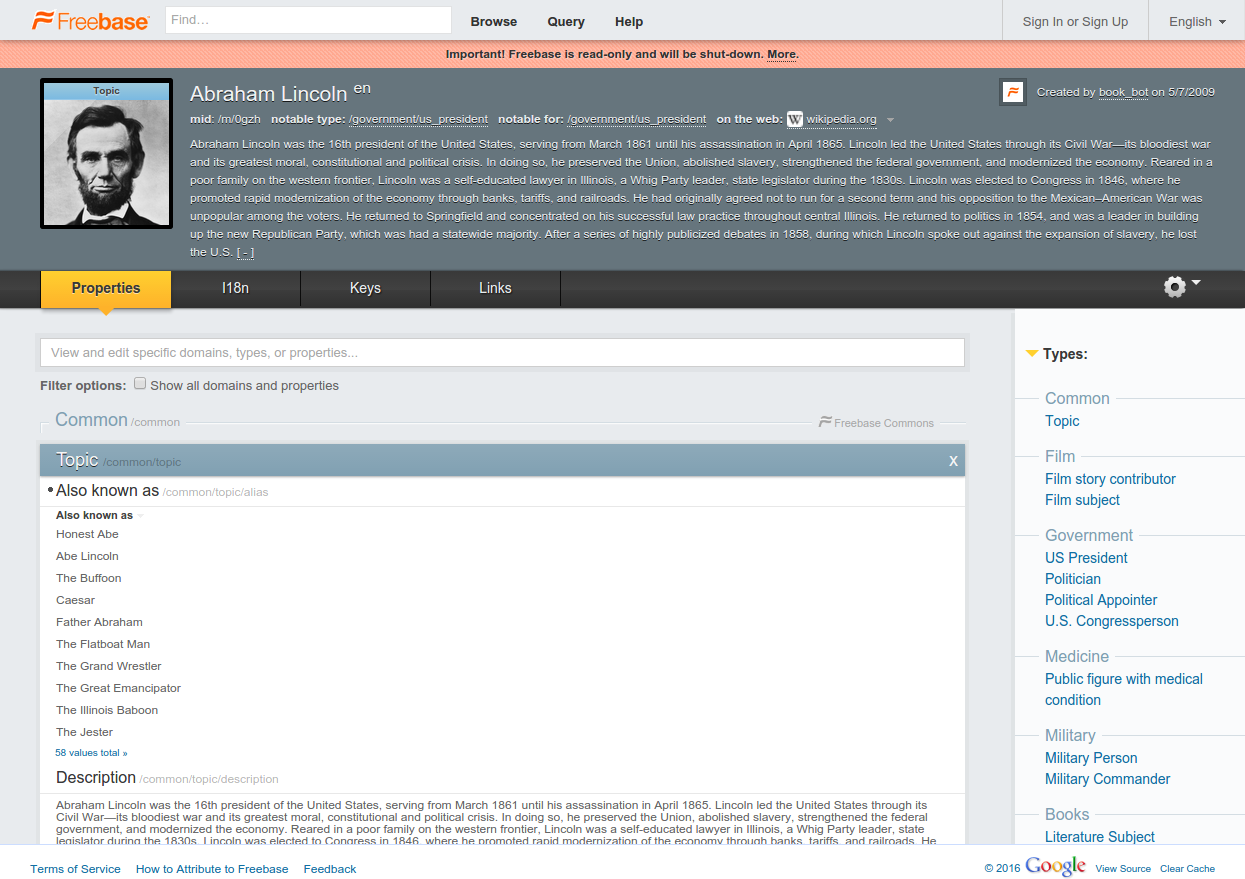
\includegraphics[width=\textwidth]{freebaseabe}
  \end{center}
\end{frame}

\begin{frame}[fragile]{WebQuestions (Berant, 2013)} 
\textbf{Questions:}
\begin{itemize}
\item what high school did president bill clinton attend?
\item what form of government does russia have today?
\item what movies does taylor lautner play in?
\end{itemize}
\textbf{Answers:}
\begin{itemize}
\item Hot Springs High School \url{http://www.freebase.com/view/en/bill_clinton}
\item Constitutional republic \url{http://www.freebase.com/view/en/russia}
\item  Eclipse, Valentine's Day, The Twilight Saga: Breaking Dawn -   Part 1, New Moon \url{http://www.freebase.com/view/en/taylor_lautner}
\end{itemize}
\end{frame}

\begin{frame}[fragile]{Freebase Triples}
  \begin{center}
    (subject, relationship, object)
  \end{center}

\begin{verbatim}
What American cartoonist is the creator of Andy Lippincott? 
(andy lippincott, character created by, garry trudeau)

Which forest is Fires Creek in?
 (fires creek, containedby, nantahala national forest)

What is an active ingredient in childrens earache relief ? 
(childrens earache relief, active ingredients, capsicum)

What does Jimmy Neutron do? 
(jimmy neutron, fictional character occupation, inventor)
\end{verbatim}
\end{frame}

\begin{frame}
  Method:
  \begin{itemize}
  \item Embed Freebase entities and relations.
    \air

  \item Learn mapping between question words and freebase
    \air 

  \item Include large amounts of semi-supervision to learn embeddings

  \end{itemize}
\end{frame}

\begin{frame}
  \begin{quote}
    Existing approaches for QA from
KBs use learnable components to either transform
the question into a structured KB query
(Berant et al., 2013) or learn to embed questions
and facts in a low dimensional vector space and retrieve
the answer by computing similarities in this
embedding space (Bordes et al., 2014a).
  \end{quote}
\end{frame}

\begin{frame}
  Start with memory containing all freebase triples
  \begin{itemize}
  \item[I] Input the questions
  \item[G] Compute continuous bag of n-grams
  \item[O] Score all triples based on embeddings
    \[j^* = \argmax_j s(\boldx, \bolds_j) = \argmax_j \cos(\boldx, \bolds_j)\]
  \item[R] Respond with the matched triple result.
  \end{itemize}
\end{frame}


\begin{frame}
  \begin{quote}
    Hence, in this paper, we introduce a new dataset of much larger
    scale for the task of simple QA called SimpleQuestions.  2 This
    dataset consists of a total of 108,442 questions written in
    natural language by human English-speaking annotators each paired
    with a corresponding fact from FB2M that provides the answer and
    explains it.
  \end{quote}
\end{frame}



\begin{frame}
  \begin{quote}
    The term simple QA refers to the simplicity of
the reasoning process needed to answer questions,
since it involves a single fact. However, this does
not mean that the QA problem is easy per se, since
retrieving this single supporting fact can be very
challenging as it involves to search over millions
of alternatives given a query expressed in natural
language.
  \end{quote}
\end{frame}


\section{Read and Comprehend}
\begin{frame}
  \includegraphics[width=\textwidth]{cnndm}
\end{frame}


\begin{frame}
  \includegraphics[width=\textwidth]{anonda}
\end{frame}

\begin{frame}
  \begin{quote}
    The Attentive Reader can be viewed as a generalisation of the application of Memory Networks to
question answering [3]. That model employs an attention mechanism at the sentence level where
each sentence is represented by a bag of embeddings. The Attentive Reader employs a finer grained
token level attention mechanism where the tokens are embedded given their entire future and past
context in the input document.
  \end{quote}
\end{frame}

\begin{frame}{The Architecture}
  Read all bi-directional document positions 
  \begin{itemize}
  \item[I] Read source with blank
  \item[G] Run RNN over the source
  \item[O] Find source entity with best match.
  \item[R] Score match at that position.
  \end{itemize}
\end{frame}


\begin{frame}
  \includegraphics[width=\textwidth]{attenreader}
\end{frame}


\begin{frame}
  \includegraphics[width=\textwidth]{impreader}
\end{frame}


\begin{frame}
  \includegraphics[width=\textwidth]{attenread}
\end{frame}

\end{document}